\documentclass[a4paper,12pt,twoside]{article}
\usepackage[top=2.5cm,bottom=2.5cm,inner=3cm,outer=2cm, headheight=1.25cm, footskip=1.25cm]{geometry}
\usepackage{setspace}
\usepackage{fancyhdr}
\usepackage{titlesec}
\usepackage{enumitem}

\usepackage[polish]{babel}
\usepackage{pdfpages}
\usepackage{graphicx}
\usepackage{float}
\usepackage[T1]{fontenc} 
\usepackage[utf8]{inputenc} 
\usepackage{helvet} 
\renewcommand{\familydefault}{\sfdefault} 
\usepackage{amsmath}
\usepackage{chngcntr}
\counterwithin{figure}{section} 
\usepackage{amsmath}
\usepackage{tocloft}
\usepackage{nomencl}
\usepackage[normalem]{ulem}
\makenomenclature
\usepackage[nottoc]{tocbibind}
\usepackage{tocloft}
\usepackage{caption}


\newcommand{\listequationsname}{Spis równań}
\newlistof{myequations}{equ}{\listequationsname}
\newcommand{\myequations}[1]{%
    \addcontentsline{equ}{myequations}{\protect\numberline{\theequation}#1}\par
}

\captionsetup[figure]{name=Rys.}

\usepackage{minted}
\usepackage{listings}
\usepackage{lmodern}
\usepackage{hyperref}

\renewcommand*\familydefault{\sfdefault}

\pagestyle{fancy}
\fancyhead{}
\fancyhead[LO,RE]{}
\fancyfoot{}
\fancyfoot[LE,RO]{\thepage}
\fancyfoot[LO,RE]{}
\renewcommand{\headrulewidth}{0pt}

\setlength{\parindent}{0.5cm}
\setlist[itemize]{label=•,itemsep=0pt}

\titleformat{\section}{\normalfont\fontsize{16}{18}\bfseries}{\thesection}{1em}{}
\titleformat{\subsection}{\normalfont\fontsize{14}{16}\bfseries}{\thesubsection}{1em}{}
\titleformat{\subsubsection}{\normalfont\fontsize{13}{15}\bfseries}{\thesubsubsection}{1em}{}

\begin{document}
\thispagestyle{empty}


\includegraphics[width=5in]{LogoPL.png}

\begin{centering}

\vspace{1cm}

\textbf{\textit{\large{Piotr Tomczak}}}

\vspace{.1cm}

\textbf{\textit{\large{250006}}}

\vspace{1.5cm}

{\large{PRACA DYPLOMOWA}}

\vspace{.1cm}

{\large{magisterska}}

\vspace{.1cm}

na kierunku Informatyka Stosowana

\vspace{1.8cm}

\textbf{\Large{Analiza wydajnościowa środowisk uruchomieniowych JavaScript}}

\end{centering}

\vspace{3.0cm}
\begin{centering}
{Instytut Informatyki I72}\\
\end{centering}
\vspace{1.0cm}
\textbf{Promotor: dr. hab. inż Joanna Ochelska-Mierzejewska} \dotfill

\begin{centering}
(tytuł/stopień naukowy, imię i nazwisko)

~\\

\end{centering}
\textbf{Opiekun pomocniczy:*)} \dotfill

\begin{centering}
(tytuł/stopień naukowy, imię i nazwisko)

~\\

\end{centering}
\textbf{Promotor uczelni partnerskiej:**)} \dotfill

\begin{centering}
(tytuł/stopień naukowy, imię i nazwisko)

~\\

\end{centering}

\vfill

\begin{centering}
ŁÓDŹ 2024\\

\end{centering}

*	jeśli został powołany

**	w przypadku procedury uznania


\pagenumbering{roman}
\setcounter{page}{2}

\onehalfspacing

\tableofcontents

\newpage
\pagenumbering{arabic}
\setcounter{page}{1}

% Rozdziały pracy
\newpage
\section*{Streszczenie}
\addcontentsline{toc}{section}{Streszczenie}
Praca magisterska pt. Analiza wydajnościowa środowisk uruchomieniowych JavaScript, koncentruje się na szczegółowym badaniu i porównaniu najważniejszych środowisk uruchomieniowych JavaScript, które są powszechnie wykorzystywane w nowoczesnym programowaniu webowym oraz serwerowym. W szczególności analizowane są Node.js, Deno oraz Bun.

Głównym celem pracy jest zidentyfikowanie różnic, zalet i wad każdego ze środowisk oraz ocena ich przydatności w różnych scenariuszach programistycznych. Praca ma na celu dostarczenie programistom i decydentom technologicznym kompleksowej wiedzy, która pomoże im w wyborze odpowiedniego narzędzia do realizacji swoich projektów.

W pracy zastosowano kombinację metod badawczych, w tym przegląd literatury, eksperymentalne testy wydajności, analizę funkcjonalności oraz ankiety wśród programistów. Przeprowadzone eksperymenty obejmowały pomiar wydajności w różnych scenariuszach (np. obsługa dużej liczby żądań HTTP, operacje wejścia/wyjścia, przetwarzanie danych) oraz ocenę łatwości użycia i dostępności bibliotek.

Node.js - Najbardziej dojrzałe i szeroko stosowane środowisko uruchomieniowe, oferujące bogaty ekosystem bibliotek NPM oraz stabilność w produkcji. Wyróżnia się doskonałą obsługą I/O oraz wsparciem dla długoterminowych projektów.

Deno - Nowoczesne środowisko stworzone przez Ryana Dahla, twórcę Node.js, które kładzie duży nacisk na bezpieczeństwo i zgodność z nowoczesnymi standardami ECMAScript. Deno integruje TypeScript bezpośrednio, co eliminuje konieczność dodatkowej konfiguracji.

Bun - Najnowsze środowisko uruchomieniowe, skoncentrowane na wydajności i prostocie użycia. Charakteryzuje się szybkim czasem startu oraz niskim zużyciem zasobów, co czyni je obiecującym wyborem dla aplikacji wymagających wysokiej wydajności.

Przeprowadzone analizy wskazują, że każde ze środowisk ma swoje unikalne zalety i wady, które czynią je odpowiednimi dla różnych typów projektów.

\bigskip

\textbf{Słowa kluczowe}: JavaScript, Wydajność, Deno, Bun, NodeJS
\newpage

\section*{Abstract}
\addcontentsline{toc}{section}{Abstract}
The thesis entitled Performance analysis of JavaScript runtime environments focuses on a detailed study and comparison of the most important JavaScript runtime environments that are commonly used in modern web and server-side programming. In particular, Node.js, Deno and Bun are analyzed.

The main aim of the work is to identify the differences, advantages and disadvantages of each environment and to evaluate their suitability in different programming scenarios. The work aims to provide developers and technology decision makers with comprehensive knowledge to help them choose the right tool for their projects.

The work used a combination of research methods, including a literature review, experimental performance testing, functionality analysis and developer surveys. The experiments conducted included measuring performance in various scenarios (e.g. handling a large number of HTTP requests, input/output operations, data processing) and assessing the ease of use and accessibility of the libraries.

Node.js - The most mature and widely used runtime environment, offering a rich ecosystem of NPM libraries and stability in production. It stands out for its excellent I/O support and support for long-term projects.

Deno - A modern runtime environment created by Ryan Dahl, the creator of Node.js, with a strong focus on security and compliance with modern ECMAScript standards. Deno integrates TypeScript directly, eliminating the need for additional configuration.

Bun - The latest runtime environment, focused on performance and ease of use. It features fast start-up times and low resource consumption, making it a promising choice for high-performance applications.

The analyses conducted indicate that each environment has its own unique advantages and disadvantages that make them suitable for different types of projects.

\bigskip

\textbf{Keywords}: JavaScript, Performance, Deno, Bun, NodeJS


\newpage
\section*{Wstęp}
\addcontentsline{toc}{section}{Wstęp}

\subsection*{Problematyka}
\addcontentsline{toc}{subsection}{Problematyka}
W czasach, których żyjemy jesteśmy przyzwyczajeni do niemalże natychmiastowego dostępu do informacji. Aby zapewnić ciągły dostęp do informacji, konieczne jest uwzględnienie serwerów, które posiadają dostęp do tych danych. Te serwery często operują w różnych środowiskach uruchomieniowych.

Specjalnie dla sieci \nomrefpage{WWW}, został stworzony język JavaScript, który miał być wykorzystywany w przeglądarkach. Wydajność samego języka na samym początku pozostawiała dużo do życzenia, jednakże obecnie jest zdecydowanie szybszy. Obecnie język stał się językiem ogólnego użytku, jest używany nie tylko do tworzenia interakcji z przeglądarką, a także jako serwer wysyłający zapytania \nomrefpage{HTTP} do użytkowników. Przeprowadzono badania \cite{comparison_of_servers}, które wykazują, że Node pozwala na zwiększenie przepustowości serwera, wykorzystujące operacje wejścia/wyjścia. W wyżej wymienionych badań wykazano, iż ilość rdzeni ma duży wpływ na wydajność samego serwera, spowodowane jest to architekturą samego języka oraz braku wielowątkowości języka. 

Twórcy silnika V8, porównują swoją wydajność za pomocą autorskich testów wydajnościowych \cite{ten_years_of_v8_chromium} \cite{ten_years_of_v8}. Testy te są udostępniane również dla innych przeglądarek, co pozwala porównać inne silniki do V8. Test ten określa wydajność za pomocą punktów, które pozwalają ustalić, czy wydajność silnika zmieniła się w przeciągu roku. Poniższy rysunek przedstawia wynik rozwoju silnika na przestrzeni lat 2010-2018.

\begin{figure}[h]
  \centering
  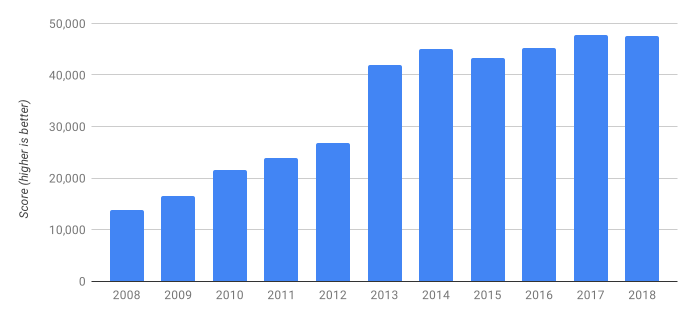
\includegraphics[width=0.9\textwidth]{Figures/v8_bench_2010_2018.png}
  \caption{Wynik przeprowadzonych testów silnika JavaScript 2010-2018}
  \label{fig:performance_v8}
\end{figure}

Na przestrzeni lat środowiskiem, które przodowało i zostało najczęściej adoptowane było środowisko NodeJS. Tą zależność pokazuje coroczna ankieta \textit{State Of Js} \cite{State_of_js:2021} \cite{State_of_js:2022}, która zbiera wyniki od deweloperów. Deweloperzy odpowiadają czy znają daną technologię, czy używali jej w przeszłości. W tej ankiecie możemy zauważyć, że na przestrzeni lat pojawili się konkurenci dla NodeJS, tymi alternatywami są Deno i Bun. Jeżeli porównamy wyniki z 2022 roku oraz 2021, możemy zauważyć, że Deno wzmocniło swoją pozycje na rynku. Deweloperzy zaczęli coraz częściej korzystać z nowej technologi. W ankiecie \textit{State Of Js} z wymienionych powyżej lat nie możemy jednak otrzymać informacji o środowisku nazwanym Bun jest to spowodowane wydaniem wersji 1.0 we wrześniu 2023.

Wymieniona powyżej ankieta mówi tylko o znajomości oraz popularności danego środowiska, aby dowiedzieć się jak dokładnie wygląda praca w danym środowisku musimy wykonać szereg działań, aby przekonać się o jego wydajności. Powstała duża liczba artykułów, które poruszały temat wydajności danego środowiska, jednak nie jesteśmy w stanie stwierdzić, jakie testy przeprowadził twórca artykułu. Dodatkowo nie są one udostępnione dla czytelnika artykułu.

Obecnie, duża ilość aplikacji webowych jest tworzona w języku JavaScript, co pozwala na tworzenie aplikacji zarówno po stronie klienta, jak i serwera. W związku z tym, że język ten jest używany w różnych środowiskach, konieczne jest przeprowadzenie badań, które pozwolą na określenie wydajności danego środowiska. Taka ewaluacja pozwoli na wybór odpowiedniego środowiska do tworzenia aplikacji, które będą wykorzystywane w różnych celach oraz na wskazanie zalet oraz wad danego środowiska, co pozwala na udoskonalenie wydajności środowisk.  

\subsection*{Cel pracy}
\addcontentsline{toc}{subsection}{Cel pracy}
Celem niniejszej pracy przeprowadzenie badań nt. obecnie występujących środowisk uruchomieniowych oraz analiza wad oraz zalet środowisk. W tym celu zidentyfikowano różne środowiska uruchomieniowe, a następnie opracowano zestaw testów wydajnościowych, które pozwoliły na ocenę działania każdego środowiska pod kątem wykorzystywanych algorytmów. Dla przedstawienia wyników testów  została przygotowana aplikacja webowa, której zadaniem jest prezentowanie wyników testów w oparciu o React \cite{React} oraz FastAPI \cite{FastAPI}. Dla każdego testu zostanie przygotowany wykres z czasami wykonania dla danej iteracji, ilość pamięci wykorzystanej wraz z zużyciem procesora w trakcie wykonywania testu. Dla testu związanego z żądaniami \nomrefeq{HTTP} został rozszerzony o statystyki, które posiada program oha \cite{oha}.

\subsection*{Zakres pracy}
\addcontentsline{toc}{subsection}{Zakres pracy}
Zakres pracy obejmuje zbudowanie testów wydajnościowych w językach JavaScript oraz Typescript dla wybranych środowisk uruchomieniowych JavaScript oraz przedstawienie wyników testów oraz ich analizę. Umożliwiająca analizę wyników testów została zbudowana aplikacja w oparciu o React \cite{React} oraz FastAPI \cite{FastAPI} aplikacja webowa, która przestawia dane w formie wykresu wraz z danymi o zużyciu procesora oraz pamięci \nomrefeq{RAM}.

\subsection*{Układ pracy}
\addcontentsline{toc}{subsection}{Układ pracy}
W tej sekcji znajduje się opis poszczególnych rozdziałów:
\begin{enumerate}
  \item Wstęp - rozdział, który przedstawia problematykę, cel oraz zakres pracy.
  \item Przegląd środowisk uruchomieniowych - rozdział, w którym opisane są wybrane środowiska uruchmomieniowe.
  \item Metodologia badań - rozdział, w którym została przedstawiona metodologia przeprowadzonych badań.
  \item Eksperymenty - rozdział, w którym zostały przedstawione wyniki przeprowadzonych badań.
  \item Dyskusja wyników - rozdział, w którym przedstawiona analiza wyników badań.
  \item Podsumowanie - rozdział, w którym zostały przedstawione wnioski dotyczące wyników.
\end{enumerate}


\newpage
\section*{Cel i zakres pracy}
\addcontentsline{toc}{section}{Cel i zakres pracy}


\newpage
\section{Przegląd środowisk uruchomieniowych}\label{env}
Do czasów powstania pierwszego środowiska uruchomieniowego JavaScript, możliwość uruchomienia programów ograniczał się do przeglądarki. Przeglądarki nie pozwalały na dostęp do pików, co nie pozwalało zapisywać dodatkowych plików na maszynie klienta. W ten sposób powstało pierwsze środowisko uruchomieniowe JavaScript w 2009, czyli NodeJS.

Środowiska uruchomieniowe pozwalają na uruchomienie skryptów JavaScriptu poza przeglądarką. Pozwoliło to językowi JavaScript stać się językiem generalnego użycia, co dla programistów stworzyło możliwość tworzenia aplikacji desktopowych, pozwoliło także na tworzenie API. Atutem powstałego w 2009 roku środowisko był asynchroniczny dostęp do systemu plików, pozwoliło to na optymalizacje operacji wejścia/wyjścia dla dużych skalowalnych aplikacji webowych.

Po upływie czasu zauważono, że NodeJS nie jest na tyle szybkim językiem do tworzenia serwerów, które mogły przekazywać informacje poprzez żądania HTTP. Stworzono także menadżera paczek, który pozwalał z jednego repozytorium pobierać paczkę, która umożliwiała uzupełnić braki samego środowiska. W czasie rosnącej popularności także zauważono, że rośnie liczba bibliotek, które korzystały z słabych punkty samego środowiska, dzięki którym pozyskano wrażliwe dane.

W odpowiedzi na narastające problemy związku działanie środowiska NodeJSm jego wolnym działaniem, zaczęto prace nad nowym bezpieczniejszym oraz wydajniejszym środowiskiem uruchomieniowym czyli Deno. Początkowo zostało zbudowane w oparciu o język Go, który został zamieniony na język Rust. Samo środowisko korzystało z silnika JavaScript stworzonego przez Google czyli V8. Twórcy Deno chcieli, aby paczki były dostępne pod linkiem, co oznacza szybsze przejście do samych pakietów. Dodatkowo Deno wprowadziło natywne wsparcie do TypeScript'a, pozwoliło to na statyczne typowanie samych bibliotek oraz zewnętrznych pakietów. Wersja 1.0 Deno, została wydana 13 maja 2020 roku.

Środowiska zostały wybrane na podstawie corocznej ankiety State of JS \cite{State_of_js:2022}, w której programiści wybierają narzędzia, które są przez nich najczęściej używane. Na liście z 2022 roku, można zauważyć, że nie został wymienione środowisko Bun,  spowodowane jest to wydanie wersji 1.0 we wrześniu 2023 roku. Możemy jednakże zauważyć, że Bun pojawia się w pracach \cite{NodeAndBun}, które analizują wydajność NodeJs oraz Bun.

Bun jako najmłodszy reprezentant środowisk wyróżnia się od pozostałych środowisk swoją szybkością, wbudowanym w sam silnik menadżer pakietów i bundler, co ułatwiło deweloperom kompresowanie samych aplikacji webowych. Środowisko to zostało napisane w języku Zig, dzięki czemu zawdzięcza swoją szybkość.

W tym rozdziale znajduje się opis wybranych do badań środowisk uruchomieniowych JavaScript.

\subsection{NodeJS}
NodeJs jest to powstałe w 2009 środowisko uruchomieniowe, które pozwoliło na znaczne rozwinięcie samego środowiska języka JavaScript o dodatkowe funkcjonalności. Środowisko zostało oparte o silnik V8 od Google, które pozwoliło na uruchamianie kodu poza przeglądarką, które było do powstania środowiska niemożliwe. Wprowadziło to także możliwość tworzenia dynamicznych stron, co pozwoliło na rozwój bibliotek związanych z tworzeniem widoków. Aktualnie środowisko jest rozwijane przez OpenJs Fundation, sama organizacja wprowadza zmiany do samego środowiska np. obsługa zmiennych środowiskowych pobieranych z pliku.

Środowisko zostało zbudowane o paradygmat zdarzeniowy, stosuje się w nim pętle zdarzeniową, która nasłuchuje konkretnych zdarzeń, a następnie zdarzenia, które są umieszczone w stosie zdarzeń są wykonywane w kolejności FIFO. \cite{event_loop} Przedstawioną architekturę przedstawiono na Rysunku \ref{fig:eventLoop}.

\begin{figure}[h]
  \centering
  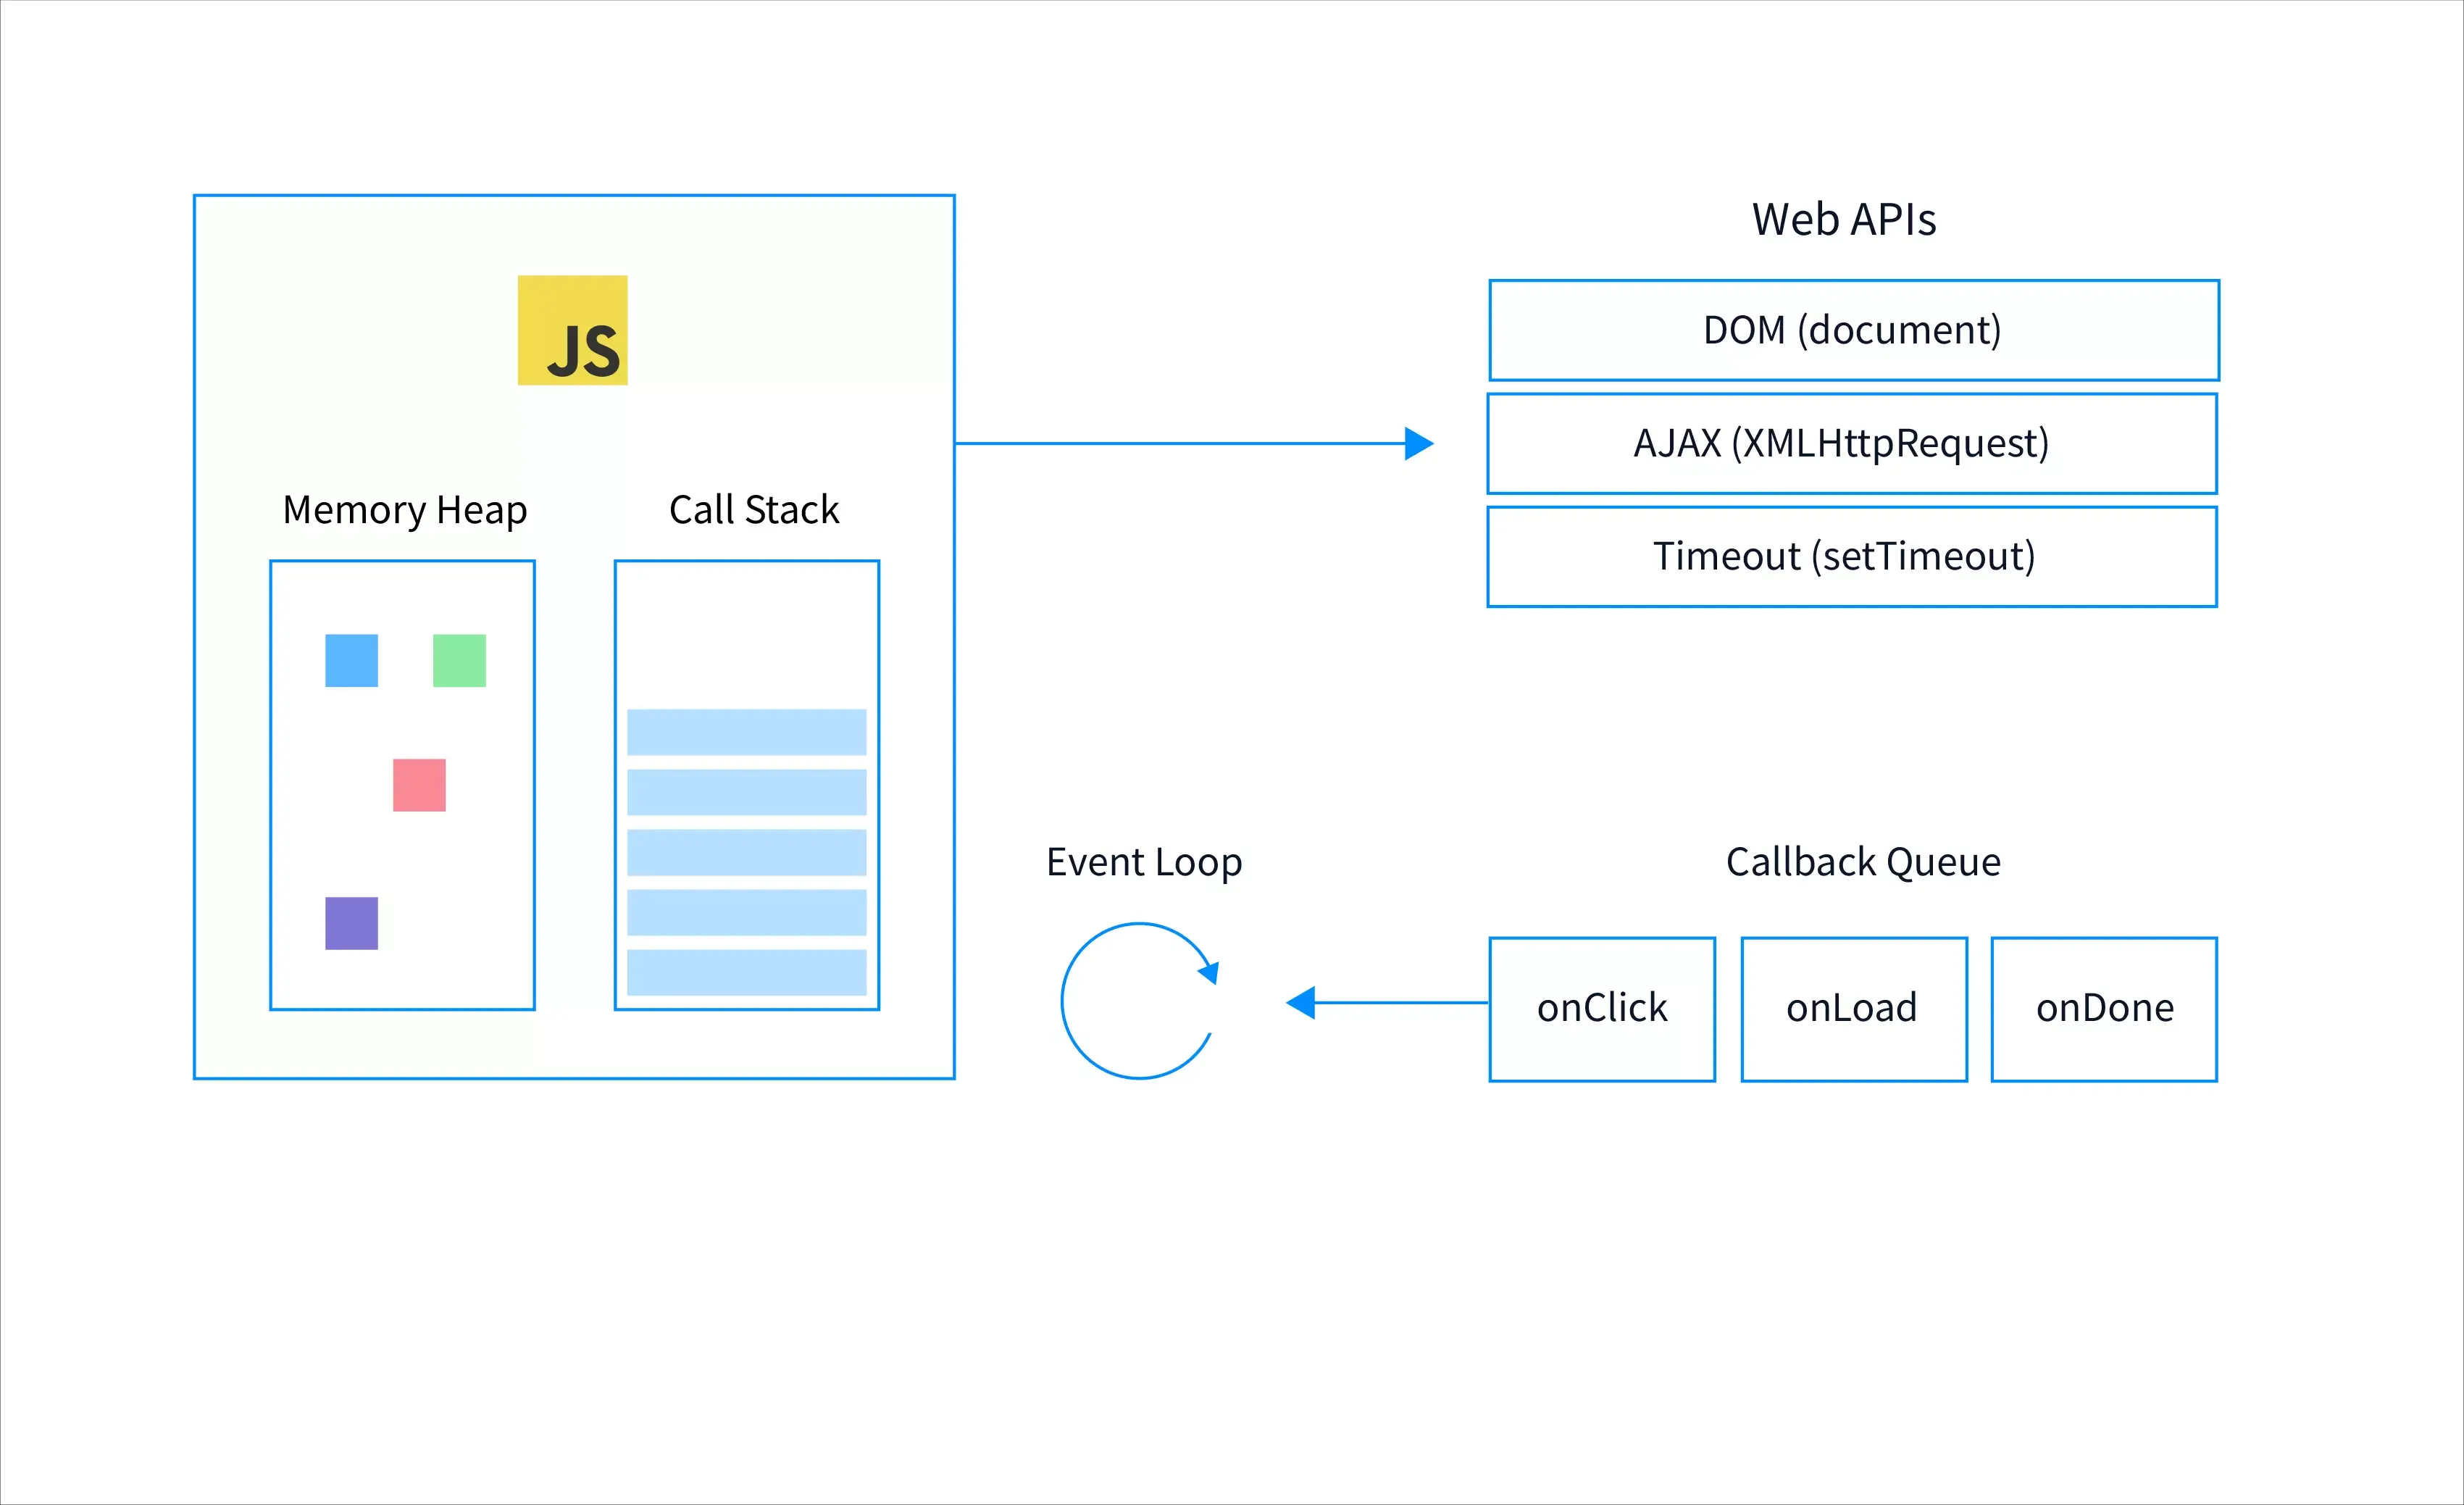
\includegraphics[width=0.9\textwidth]{Figures/eventLoop.png}
  \caption{Architektura zdarzeń}
  \label{fig:eventLoop}
\end{figure}

Zastosowanie powyższej architektury pozwoliło na wprowadzenie asynchronicznej obsługi operacji wyjścia wyjścia. Dzięki tej architekturze, NodeJs jest środowiskiem, w którym produkuje się skalowalne aplikacje internetowe. Środowisko to zostało rozwijane, gdzie dodatkowo wprowadzono moduły odpowiedzialne za funkcje kryptograficzne, funkcje odpowiedzialne za sieci oraz obsługę binarnych danych.

Środowisko posiada własny menadżer paczek, które są przeznaczone dla środowiska nazywający się npm. Npm został zaprezentowany w 2010 roku, rok od powstania samego środowiska. Korzystając z menadżer, deweloperzy mogą udostępniać biblioteki zrobione specjalnie pod NodeJs. Obecnie jest zarejestrowane 2.1 miliona bibliotek \cite{npm}, które znajdują się na w npm. Na przestrzeni czasu, można zauważyć, że Npm nie jest wydajnym menadżerem, dlatego też powstały alternatywy do npm takie jak: yarn \cite{yarn} oraz pnpm \cite{pnpm}. 

W środowisku możemy pisać w kilku językach, niestety nie odbywa się to bez dodatkowej konfiguracji projektu. Sam NodeJs odczytuje tylko i wyłącznie programy transpilowane lub napisane w JavaScript. Na dzień dzisiejszy dzień środowisko wspiera transpilowanie w kilku języków takich jak: CoffeeScript, Dart, TypeScript oraz ClojureScript.

\subsection{Deno}
Deno jest to środowisko uruchomieniowe, które zostało podobnie jak NodeJs zbudowane na podstawie silnika V8 od Google. Współautorem środowiska jest Ryan Dahl, który jest współtwórcą Deno. Deno jako środowisko spełnia rolę menadżera paczek, który pozwala na pobieranie paczek z repozytorium. W przeciwieństwie do NodeJs, Deno nie posiada menadżera paczek, co pozwala na szybsze pobieranie paczek. Wszystkie paczki są dostępne pod linkiem, co pozwala na szybsze pobieranie paczek.

Dzięki bazowaniu na silniku V8 oraz przepisaniu części funkcjonalności za języka Rust, pozwoliło na zwiększenie wydajności samego silnika. Wydajność samego Deno została zbadana w pracy \cite{deno_performance}, w której porównano wydajność samego środowiska z NodeJs. W pracy wykazano, że Deno jest szybsze od NodeJs, co pozwala na zwiększenie wydajności samego środowiska. W tej pracy sprawdzono wydajność wysyłanych żądań HTTP, w której wykazano, że Deno jest szybsze od NodeJs. Rysunek \ref{fig:deno_vs_node} przedstawia wyniki porównania wydajności Deno oraz NodeJs.

\begin{figure}[H]
  \centering
  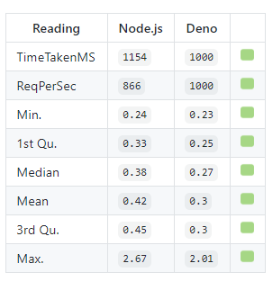
\includegraphics[width=0.52\textwidth]{Figures/deno_performance.png}
  \caption{Wyniki testu wydajnościowego Deno oraz NodeJs \cite{deno_performance}}
  \label{fig:deno_vs_node}
\end{figure}

Deno jako środowisko jest bezpieczniejsze od NodeJs, co pozwala na ograniczenie dostępu do plików, co pozwala na zwiększenie bezpieczeństwa samego środowiska. W NodeJs, dostęp do plików jest nieograniczony, co pozwala na dostęp do wszystkich plików na maszynie. W Deno, dostęp do plików jest ograniczony, co pozwala na dostęp do plików, które są wskazane w pliku konfiguracyjnym. Należy także wspomnieć, iż Deno także nie zezwala na ruch sieciowy bez wskazania właściwej flagi, co pozwala na zwiększenie bezpieczeństwa samego środowiska.

Deno jako środowisko posiada wbudowane wsparcie dla TypeScript, co pozwala na statyczne typowanie samych bibliotek oraz zewnętrznych pakietów. W NodeJs, musimy zainstalować dodatkowe paczki, które pozwolą na statyczne typowanie. W Deno, nie musimy instalować dodatkowych paczek, co pozwala na szybsze tworzenie aplikacji.

Deno jako środowisko posiada wbudowany bundler, co pozwala na kompresowanie samej aplikacji. W NodeJs, musimy zainstalować dodatkowe paczki, które pozwolą na kompresowanie samej aplikacji. W Deno, nie musimy instalować dodatkowych paczek, co pozwala na szybsze tworzenie aplikacji.

Samo środowisko udostępnia także wbudowane narzędzia pozwalające na tworzenie aplikacji webowych w oparciu o składnie JSX bądź TSX. Dzięki czemu środowisko jest rozszerzone, deweloperzy nie muszą tworzyć repozytoriów odpowiedzialnych tylko za widoki przedstawione na stronie. Pozwala to na tworzenie jednej wspólnej bazy kodowej, co pozwala na szybszy rozwój aplikacji.

Misją samego środowisko jest ujednolicanie bazy kodowej napisanych w tym środowisku. Z tego powodu Deno posiada swój własny formater kodu, który pozwala na pozbycie się dodatkowych pakietów odpowiedzialnych za formatowanie kodu. 

\subsection{Bun}
Bun \cite{bun} jest to najmłodsze środowisko uruchomieniowe, stworzone przez Jarreda Summera. Wersja 1.0 została zaprezentowana we wrześniu 2023 roku. Środowisko to zostało zbudowane na podstawie silnika JavaScript WebKit, jest to rozwiązanie od firmy Apple wykorzystywane w przeglądarce Safari.

Sam autor środowiska twierdzi, że środowisko jest szybsze od NodeJs oraz Deno, co pozwala na zwiększenie wydajności samego środowiska. W pracy \cite{NodeAndBun} porównano wydajność samego środowiska z NodeJs oraz Bun. W pracy wykazano, że Bun jest szybsze od NodeJs, co pozwala na zwiększenie wydajności samego środowiska. W tej pracy sprawdzono wydajność samego środowiska, w której wykazano, że Bun jest szybsze od NodeJs. Jednakże ta praca pokazuje w najbardziej wydajność, tylko i wyłącznie w liczbie żądań na sekundę. Rysunek \ref{fig:bun_vs_node} przedstawia wyniki porównania liczby żądań HTTP przy założonej liczby współbieżnych połączeń z serwerem połaczeniach Bun oraz NodeJs.

\begin{figure}[H]
  \centering
  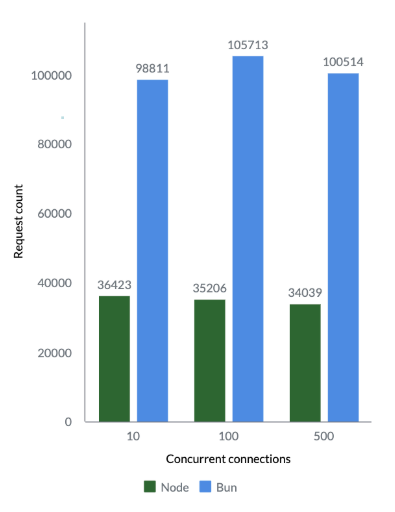
\includegraphics[width=0.47\textwidth]{Figures/bun_bench_node.png}
  \caption{Wyniki testu wydajnościowego Bun oraz NodeJs \cite{bun_test}}
  \label{fig:bun_vs_node}
\end{figure}

Sam twórca opracował testy wydajnościowe, sprawdzające wydajność środowiska ich rezultaty są opublikowane na stronie \cite{bun_test}. Autor korzystał wbudowanych w silniki metod, które odpowiadają za SSR (\textit{ang. Server Side Rendering}), co imituje środowisko przeglądarki. Jednakże możemy zauważyć, że jest to prosta strona, która zawiera tylko tekst. W testach wydajnościowych sprawdzono wydajność samego środowiska, w których wykazano, że Bun jest szybsze od NodeJs. Rysunek \ref{fig:bun_bench} przedstawia wyniki porównania liczby żądań HTTP na sekundę.

\begin{figure}[H]
  \centering
  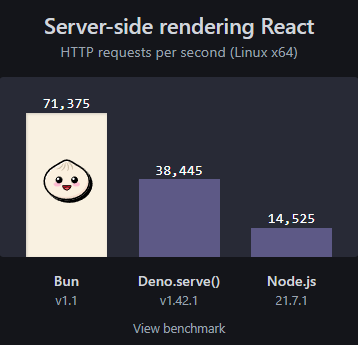
\includegraphics[width=0.47\textwidth]{Figures/bun_bench.png}
  \caption{Wyniki testu wydajnościowego Bun oraz NodeJs \cite{bun_test}}
  \label{fig:bun_bench}
\end{figure}

To co wyróżnia środowisko od pozostałych to wbudowany menadżer pakietów, który pozwala na integracje z npm \cite{npm} oraz pozwala na importowanie paczek z samego NodeJs. Pozwala to na integracje z powstałymi już projektami w NodeJs. Samo środowisko też nie potrzebuje pliku \textit{package.json} \cite{package_structure}, które w NodeJs jest wymagane. Samo środowisko tworzy jeden plik odpowiedzialny za wszystkie zależności wykorzystywane w projekcie.

Sprawdzenie jakości kodu jest ułatwione, dla użytkowników środowiska ze względu na wbudowane środowisko testowe. Pozwala to na zrezygnowanie z dodatkowych bibliotek odpowiedzialnych za tworzenie testów. Samo środowisko posiada asercję oraz dodatkowe funkcje, które pozwalają na tworzenie testów jednostkowych. Niektóre funkcje pozwala na niewykonywanie testów w zależności od warunków dla na przykład wyłączenie danego testu w zależności od architektury danego systemu. W dokumentacji znajduję się przykład samej asercji, który przedstawiono na Listingu \ref{lst:bun_assert}.

\begin{centering}
  \begin{lstlisting}[caption={Przykład asercji w środowisku Bun},label={lst:bun_assert},captionpos=b]
    const macOS = process.arch === "darwin";
    test.skipIf(macOS)("runs on non-macOS", () => {
      // runs if *not* macOS
    });
  \end{lstlisting}
\end{centering}




\newpage
\section{Metodologia badań}
W tym rozdziale przedstawiono metodologię przeprowadzonych badań, środowisko testowe oraz wybrane algorytmy do badań środowisk uruchomieniowych.

\subsection{Środowisko testowe}
Do przeprowadzenia testów został wykorzystany system operacyjny Linux Ubuntu 22.04.03, zainstalowany w (ang. \textit{ang. Windows Subsystem for Linux}). Wybór ten dodatkowo jest podyktowany faktem iż do momentu pisania niniejszej pracy, środowisko Bun nie udostępniło oficjalnego wsparcia dla systemu Windows.

Wybór powyższego systemu jest podyktowany faktem, że jest to system, na którym wybrane środowiska są najczęściej uruchamiane. Badanie wykonane w 2015 roku, pokazuje iż większość osób odpowiedzialnych za administrowanie aplikacjami webowymi korzysta z systemu Linux \cite{performance_comparison_linux}. Kolejnym badaniem przeprowadzonym w 2021 roku, pokazało iż sam system jest bardziej wydajny niż Windows Server \cite{web_server_performance}. Badania także pokazało, że większość serwerów internetowych działa na systemie Linux. W związku z tym, wybór systemu Linux jest uzasadniony.

Wymienione środowiska posługują się swoimi implementacjami programów umożliwiających uruchamianie programów opartych o Javascript, staje się to problematyczne w przypadku użycia języka TypeScript. Aby uruchomić skrypty napisane za pomocą tego języka TypeScript należy je stranspilować do języka Javascript. W przypadku NodeJs, powstały odpowiednie paczki tj.: \textit{ts-node} \cite{ts_node}, \textit{tsx} \cite{tsx}. Potrafią one przetworzyć pliki napisane w TypeScript do Javascript. W przypadku Deno oraz Bun, ta funkcjonalność jest wbudowana w środowisko, pozwala to na zrezygnowanie z dodatkowych narzędzi.

Środowiska także inaczej podchodzą do zapisu plików na urządzeniach. We wszystkich środowiskach można zapisać oraz odczytać plik za pomocą metod synchronicznych jak i asynchronicznych. Środowisko Bun udostępnia swoją implementacje zapisy oraz odczytu wykorzystując swoje metody asynchroniczne. Dodatkowym atutem samego środowiska Bun jest możliwość użycia bibliotek, które są odpowiednikiem dla tych dostępnych w NodeJs. W przypadku Deno, zapis oraz odczyt odbywa się za pomocą dekoderów oraz enkoderów, które odczytują tekst w zadanym formacie.

\section{Wybrane narzędzi i algorytmy}
W tym rozdziale znajdują się algorytmy wykorzystane w testach wydajnościowych dla każdego środowiska uruchomieniowego. Wraz z podaniem opisu algorytmu, znajduje się także opis zastosowania algorytmu w praktyce.

\subsection{Algorytmy sortowania}
W testach zostały wykorzystane trzy algorytmy sortowania, które są najczęściej wykorzystywane w praktyce. Sortowanie jako metoda jest używana w wielu zastosowaniach, takich jak sortowanie danych w bazach danych, sortowanie danych w aplikacjach webowych, a także w algorytmach wyszukiwania. W teście sortowania został przeprowadzone testy na losowo wybranych liczbach całkowitych.

Liczby całkowite zostały wylosowane za pomocą generatora liczb całkowitych. Do samej implementacji generatora liczb całkowitych posłużył pakiet \textit{Math}, który jest dostępny w języku JavaScript. Generator został zaimplementowany tak, aby losował liczby w zależności od zadanego rozmiaru tablicy.

Każdy z algorytmów charakteryzuje się inną złożonością obliczeniową, co wpływa na czas sortowania danych. Możemy to zauważyć w pracy \cite{sorting}, gdzie pokazywane są czasy poszczególnych algorytmów sortowania. W tabeli \ref{tab:sorting_complexity} przedstawiono złożoności obliczeniowe dla poszczególnych algorytmów.

\begin{table}[h]
  \centering
  \begin{tabular}{|l|l|l|l|}
  \hline
  \textbf{Algorytm Sortowania} & \textbf{Optymistyczna} & \textbf{Średnia} & \textbf{Pesymistyczna} \\ \hline
    Bubble Sort & $O(n)$ & $O(n^2)$ & $O(n^2)$ \\ 
    \hline
    Quick Sort & $O(n log n)$ & $O(n log n)$ & $O(n^2)$ \\ 
    \hline
    Radix Sort & $O(nk)$ & $O(nk)$ & $O(nk)$ \\
    \hline
  \end{tabular}
  \caption{Złożoność obliczeniowa dla algorytmów sortowania}
  \label{tab:sorting_complexity}
\end{table}

\subsubsection{Sortowanie bąbelkowe (\textit{ang. Bubble Sort})}
Sortowanie bąbelkowe (\textit{ang. Bubble Sort}) to jeden z najprostszych algorytmów sortowania. Algorytm ten działa poprzez porównywanie dwóch sąsiadujących elementów i zamianę ich miejscami, jeśli są w niewłaściwej kolejności. Złożoność obliczeniowa algorytmu w pesymistycznym wypadku wynosi $O(n^2)$.

Działanie algorytmu można określić w kilku krokach:
\begin{enumerate}
  \item Przejdź przez tablicę od początku do końca.
  \item Dla każdego elementu, sprawdź czy sąsiedni element jest mniejszy od obecnego.
  \item Jeśli sąsiedni element jest mniejszy, zamień miejscami obecny element z sąsiednim.
  \item Powtarzaj kroki 1-3, aż tablica zostanie posortowana.
\end{enumerate}

Algorytm ten jest jednym z najwolniejszych algorytmów sortowania, jednakże jest on prosty w implementacji. W przypadku małych zbiorów danych, algorytm ten jest wystarczający, jednakże w przypadku dużych zbiorów danych, algorytm ten może być bardzo wolny. W najlepszym wypadku, gdy tablica jest już posortowana złożoność obliczeniowa wynosi $O(n)$, co oznacza, że algorytm ten jest szybki w przypadku posortowanych danych.

\subsubsection{Sortowanie szybkie (\textit{ang. Quick Sort})}
Quick Sort to jeden z najpopularniejszych i najwydajniejszych algorytmów sortowania ogólnego przeznaczenia. Został opracowany przez Tony'ego Hoare'a w 1960 roku. Algorytm działa na zasadzie "dziel i zwyciężaj" (\textit{ang. divide and conquer}), co oznacza, że dzieli w przypadku testów tablicę liczb całkowitych na mniejsze tablice, które są następnie rozwiązywane rekurencyjnie.

Działanie algorytmu można określić w kilku krokach:
\begin{enumerate}
  \item Wybierz element z tablicy, który nazywamy elementem osiowym (\textit{ang. pivot}). Sam algorytm wybiera element pierwszy z tablicy jako \textit{pivot}.
  \item Podziel tablicę na dwie części: jedną z elementami mniejszymi od elementu osiowego, a drugą z elementami większymi od elementu osiowego.
  \item Rekurencyjnie posortuj obie części.
  \item Połącz obie części w jedną posortowaną tablicę.
  \item Zwróć posortowaną tablicę.
\end{enumerate}

Zaletą algorytmu jest to, że w porównaniu do algorytmu sortowanie pozycyjnego, nie wymaga on dodatkowego alokowania pamięci na tablice tymczasowe, pracuje on na oryginalnej tablicy. Można zauważyć z tabeli \ref{tab:sorting_complexity}, że algorytm w najgorszym wypadku ma złożoność obliczeniową $O(n^2)$, co oznacza, że w przypadku dużej ilości danych, algorytm ten może być wolniejszy od innych algorytmów sortowania.

\subsubsection{Sortowanie pozycyjne (\textit{ang. Radix Sort})}
Radix Sort to wydajny algorytm sortowania stosowany do porządkowania liczb całkowitych lub innych danych, które można reprezentować jako krotki o stałej długości. Algorytm działa na zasadzie sortowania pozycyjnego, czyli sortowania cyfr od najmniej znaczącej do najbardziej znaczącej (lub odwrotnie, w zależności od implementacji). Dzięki temu możliwe jest osiągnięcie bardzo dobrych wyników czasowych w przypadku dużych zbiorów danych. Złożoność obliczeniowa w przypadku sortowania pozycyjnego wynosi $O(nk)$, gdzie $n$ to liczba elementów do posortowania, a $k$ to liczba cyfr w największym elemencie zbioru.

Działanie algorytmu można określić w kilku krokach:
\begin{enumerate}
  \item Zainicjowanie samego algorytmu podając mu tablicę liczb całkowitych do posortowania.
  \item Dla każdej liczby znalezienie cyfry najmniej znaczącej i umieszczenie jej w odpowiednim kubełku.
  \item Powtarzaj krok 2 dla każdej cyfry, aż do osiągnięcia najbardziej znaczącej cyfry.
\end{enumerate}

Dzięki swojej złożoności obliczeniowej sortowanie pozycyjne jest szybkie, jednakże posiada wadę w postaci konieczności alokowania dodatkowej pamięci, aby przechowywać tymczasowe wyniki sortowania. Jednakże w przypadku danych, które nie są danymi liczbowymi należy przekształcić je na dane liczbowe, co może wpłynąć na czas sortowania. W przypadku danych, które są liczbami, algorytm ten jest jednym z najszybszych algorytmów sortowania \cite{sorting}. W testach dla ujednolicenia danych, zostały zastosowane liczby całkowite.

\subsection{Algorytmy Kodowania}
W testach został wykorzystany jeden algorytm kodowania, który jest najczęściej wykorzystywany do przesyłania danych. Wybrany algorytm kodowania jest Base64. Wykorzystywany jest on do kodowania obrazów, danych wykorzystywanych w formularzach, a także do przedstawiania plików pdf na stronach.

Algorytm możemy podzielić na trzy etapy. Pierwszym etapem jest podział danych na segmenty składające się z 24 bit. Następnie każdy z segmentów jest dzielony na cztery grupy po 6 bitów. Każda grupa zostaje mapowana na z jeden ze znaków:
\begin{itemize}
  \item Litery A-Z (26 znaków)
  \item Litery a-z (26 znaków)
  \item Cyfry 0-9 (10 znaków)
  \item Znaki "+" i "/"
\end{itemize}
W przypadku gdy grupy nie są wielokrotnością liczby 24, wtedy grupy zostają uzupełnione zerami, co przekształca się w znak \textit{=} w celu wskazania liczby dodanych bitów. Na rys \ref{fig:base64_mapping_table} przedstawiono tablicę mapowań dla algorytmu szyfrowania Base64.

\begin{figure}[H]
  \centering
  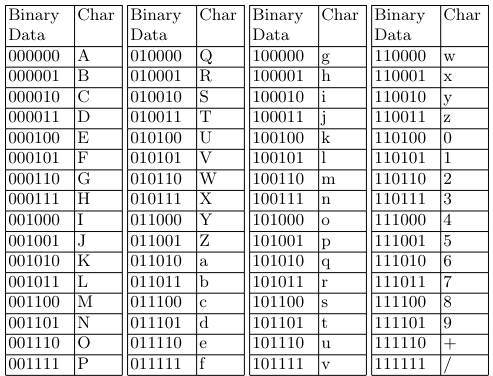
\includegraphics[width=0.6\textwidth]{Figures/base64_mapping_table.png}
  \caption{Tablica mapowań dla algorytmu szyfrowania Base64}
  \label{fig:base64_mapping_table}
\end{figure}

Algorytm ten jest przydatny do małych obrazów, jednakże w przypadku dużych obrazów, algorytm ten nie jest zalecany. Wynika to z faktu iż sam algorytm powoduje zwiększenia rozmiaru danych. Dodatkowo wykazano, że w zależności od języka programowania oraz implementacji algorytmu, czas kodowania oraz dekodowania może się różnić \cite{cryptoeprint:2022/361}.

Test został zaimplementowany z wykorzystaniem obiektu \textit{Buffer} odpowiedzialnego za kodowanie oraz dekodowanie wartości zakodowanych wiadomości. Oryginalny test wykonany przez Kostya \cite{base64_benchmark}, został zmodyfikowany, aby dodać informacje o czasie wykonywania oraz użyciu pamięci przez dane środowisko. Test ten został przeprowadzony w celu sprawdzenia jak szybko dane środowisko jest w stanie zakodować oraz odkodować dane.

\subsection{Bazy danych}
W testach została wykorzystana plikowa baza relacyjna Sqlite3. Wybór ten podyktowany jest faktem iż baza ta ma wsparcie dla wszystkich środowisk uruchomieniowych. Celem testu było zmierzenie czasu odpowiedzi bazy danych na zapytania SQL. 

W celu dodania do bazy danych przykładowych danych została wykorzystany pakiet \textit{faker-js}. Pakiet ten pozwala na generowanie obiektów z danymi losowymi. W celu przetestowania możliwości bazy danych, została opracowany model, który odzwierciedla użytkownika. Model ten składa się z pól takich jak: imię, nazwisko, płeć, opis, typ wykonywanej pracy, tytuł oraz zakres pracy. Test pozwala na specyfikowania ilości rekordów, które mają zostać dodane do bazy danych.

W przypadku NodeJs, wymagane jest aby zainstalować dodatkowy pakiet odpowiedzialny za komunikację z bazą danych. W odróżnieniu do pozostałych środowisk, które posiadają wbudowane wsparcie dla Sqlite3. Przez dodanie nowych pakietów, powiększa się rozmiar aplikacji, wpływa to na rozmiar oraz czas uruchamiania się aplikacji.

\subsection{Narzędzia pomiarowe}
W celu zmierzenia czasów wykonania poszczególnych testów, zostały wykorzystane narzędzia dostępne w języku JavaScript. Do mierzenia czasu wykonania danego testu została wykorzystana moduł \textit{performance}. Moduł ten pozwala na zapisanie czasu w postaci milisekund, co pozwala na dokładne określenie czasu wykonania danego testu. Metoda wykorzystuje obiekt \textit{DOMHighResTimeStamp}, który pozwala na określenie czasu w milisekundach z dokładnością do 5 mikrosekund.

W celu zmierzenia 

\newpage
\section{Eksperymenty}
W tym rozdziale opisane zostaną eksperymenty przeprowadzone w celu zbadania testów wydajnościowych środowisk uruchomieniowych. Testy zostały przeprowadzone na jednym komputerze wyposażonym w system operacyjny Linux, co pozwoliło na zminimalizowanie wpływu innych czynników na wyniki testów. 

\subsection{Algorytmy sortowania}
W celu zbadania wydajności danego środowiska uruchomieniowego, skonstruowana odpowiednie eksperymenty, które sprawdzają wydajność algorytmu sortowania. Wszystkie algorytmu sortowania zostały przetestowane dla każdego środowiska. W tabeli \ref{tab:sorting_experiments} przedstawiono ilość iteracji oraz ilość eksperymentów dla przeprowadzonych eksperymenty.

\begin{table}[H]
  \centering
  \begin{tabular}{|c|c|}
    \hline
    \textbf{Ilość iteracji} & \textbf{Ilość elementów} \\ \hline
    10 & 1000 \\ \hline
    100 & 1000 \\ \hline
    1000 & 1000 \\ \hline
    10 & 10000 \\ \hline
    100 & 10000 \\ \hline
    1000 & 10000 \\ \hline
  \end{tabular}
  \caption{Parametry eksperymentów}
  \label{tab:sorting_experiments}
\end{table}

\subsubsection{Wyniki - sortowanie bąbelkowe}
% 1
Na wykresie \ref{fig:bubble_sorting_e1} przedstawiono wyniki eksperymentu dla 10 iteracji oraz 1000 elementów dla algorytmów sortowania bąbelkowego napisanego w języku JavaScript. Na osi X przedstawia liczbę iteracji, na osi Y czas wykonania algorytmu w sekundach. 

\begin{figure}[H]
  \centering
  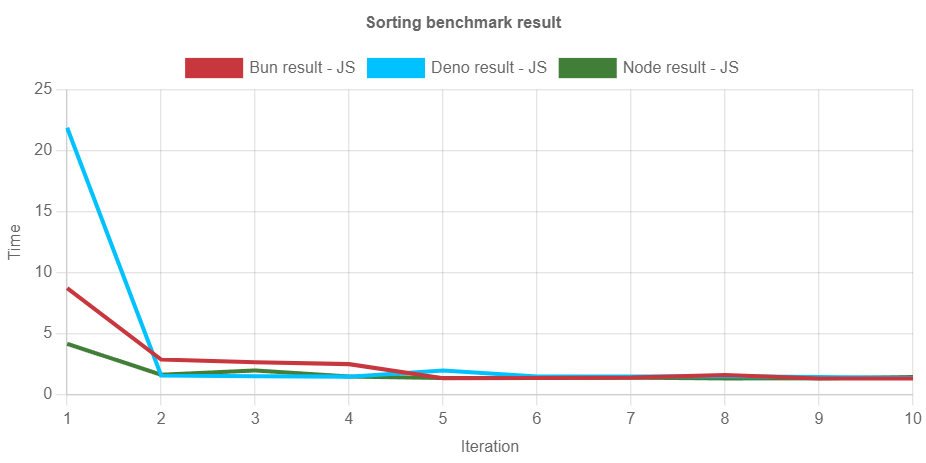
\includegraphics[width=0.7\textwidth]{Figures/sorting/bubble/e1_js.png}
  \caption{Wyniki eksperymentów dla algorytmu sortowania bąbelkowego dla 10 iteracji i 1000 elementów}
  \label{fig:bubble_sorting_e1}
\end{figure}

Na wykresie \ref{fig:bubble_sorting_e1_memory} przedstawiono wyniki eksperymentów dla algorytmu sortowania bąbelkowego dla 10 iteracji oraz 1000 elementów napisanego w języku JavaScript. Na osi X przedstawiono liczbę iteracji, natomiast na osi Y wykorzystanie pamięci w kilobytach. Jak widać, czas wykonania algorytmu rośnie wraz z ilością elementów.
\begin{figure}[H]
  \centering
  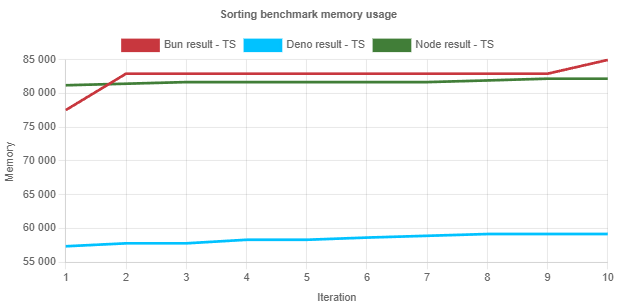
\includegraphics[width=0.7\textwidth]{Figures/sorting/bubble/e1_memory_ts.png}
  \caption{Wyniki eksperymentów dla algorytmu sortowania bąbelkowego dla 10 iteracji i 1000 elementów}
  \label{fig:bubble_sorting_e1_memory}
\end{figure}

Na wykresie \ref{fig:bubble_sorting_e1_ts} przedstawiono wyniki eksperymentu dla 10 iteracji oraz 1000 elementów dla algorytmów sortowania bąbelkowego napisanego w języku TypeScript. Na osi X przedstawia liczbę iteracji, na osi Y czas wykonania algorytmu w sekundach.

\begin{figure}[H]
  \centering
  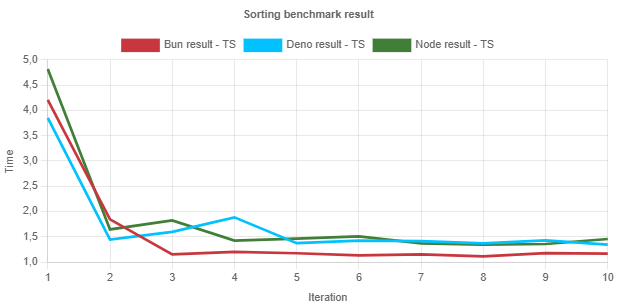
\includegraphics[width=0.8\textwidth]{Figures/sorting/bubble/e1_ts.png}
  \caption{Wyniki eksperymentów dla algorytmu sortowania bąbelkowego dla 10 iteracji i 1000 elementów}
  \label{fig:bubble_sorting_e1_ts}
\end{figure}

Na wykresie \ref{fig:bubble_sorting_e1_memory_ts} przedstawiono wyniki eksperymentów dla algorytmu sortowania bąbelkowego dla 10 iteracji i 1000 elementów napisanego w języku TypeScript. Na osi X przedstawiono liczbę iteracji, natomiast na osi Y wykorzystanie pamięci w kilobytach. Jak widać, czas wykonania algorytmu rośnie wraz z ilością elementów.
\begin{figure}[H]
  \centering
  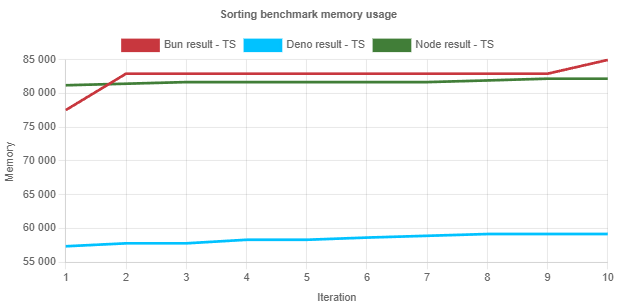
\includegraphics[width=0.8\textwidth]{Figures/sorting/bubble/e1_memory_ts.png}
  \caption{Wyniki eksperymentów dla algorytmu sortowania bąbelkowego dla 10 iteracji i 1000 elementów}
  \label{fig:bubble_sorting_e1_memory_ts}
\end{figure}

% 2
Na wykresie \ref{fig:bubble_sorting_e2} przedstawiono wyniki eksperymentu dla 10 iteracji oraz 1000 elementów dla algorytmów sortowania bąbelkowego napisanego w języku JavaScript. Na osi X przedstawia liczbę iteracji, na osi Y czas wykonania algorytmu w sekundach. 

\begin{figure}[H]
  \centering
  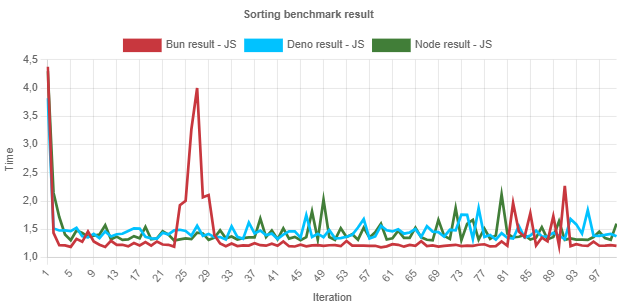
\includegraphics[width=0.8\textwidth]{Figures/sorting/bubble/e2_js.png}
  \caption{Wyniki eksperymentów dla algorytmu sortowania bąbelkowego dla 10 iteracji i 1000 elementów}
  \label{fig:bubble_sorting_e2}
\end{figure}

Na wykresie \ref{fig:bubble_sorting_e2_memory_js} przedstawiono wyniki eksperymentów dla algorytmu sortowania bąbelkowego dla 10 iteracji oraz 1000 elementów napisanego w języku JavaScript. Na osi X przedstawiono liczbę iteracji, natomiast na osi Y wykorzystanie pamięci w kilobytach. Jak widać, czas wykonania algorytmu rośnie wraz z ilością elementów.
\begin{figure}[H]
  \centering
  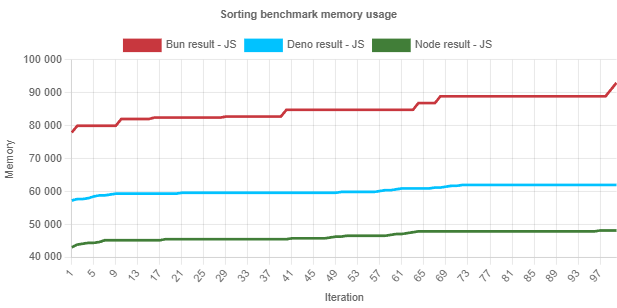
\includegraphics[width=0.8\textwidth]{Figures/sorting/bubble/e2_memory_js.png}
  \caption{Wyniki eksperymentów dla algorytmu sortowania bąbelkowego dla 100 iteracji i 1000 elementów}
  \label{fig:bubble_sorting_e2_memory_js}
\end{figure}

Na wykresie \ref{fig:bubble_sorting_e2_ts} przedstawiono wyniki eksperymentu dla 100 iteracji oraz 1000 elementów dla algorytmów sortowania bąbelkowego napisanego w języku TypeScript. Na osi X przedstawia liczbę iteracji, na osi Y czas wykonania algorytmu w sekundach. 

\begin{figure}[H]
  \centering
  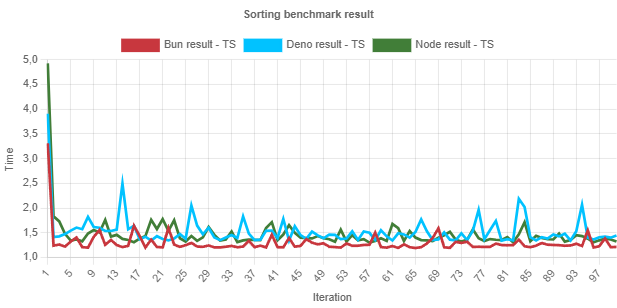
\includegraphics[width=0.8\textwidth]{Figures/sorting/bubble/e2_ts.png}
  \caption{Wyniki eksperymentów dla algorytmu sortowania bąbelkowego dla 100 iteracji i 1000 elementów}
  \label{fig:bubble_sorting_e2_ts}
\end{figure}

Na wykresie \ref{fig:bubble_sorting_e2_memory_ts} przedstawiono wyniki eksperymentów dla algorytmu sortowania bąbelkowego dla 100 iteracji i 1000 elementów napisanego w języku TypeScript. Na osi X przedstawiono liczbę iteracji, natomiast na osi Y wykorzystanie pamięci w kilobytach. Jak widać, czas wykonania algorytmu rośnie wraz z ilością elementów.
\begin{figure}[H]
  \centering
  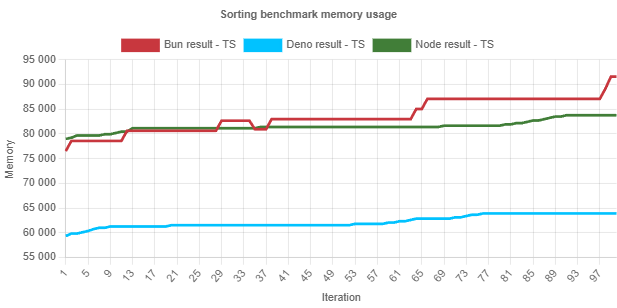
\includegraphics[width=0.8\textwidth]{Figures/sorting/bubble/e2_memory_ts.png}
  \caption{Wyniki eksperymentów dla algorytmu sortowania bąbelkowego dla 100 iteracji i 1000 elementów}
  \label{fig:bubble_sorting_e2_memory_ts}
\end{figure}

% 3
Na wykresie \ref{fig:bubble_sorting_e3} przedstawiono wyniki eksperymentów dla algorytmu sortowania bąbelkowego dla 1000 iteracji oraz 1000 elementów napisanego w języku JavaScript. Na osi X przedstawiono liczbę iteracji, natomiast na osi Y wykorzystanie pamięci w kilobytach. Jak widać, czas wykonania algorytmu rośnie wraz z ilością elementów.
\begin{figure}[H]
  \centering
  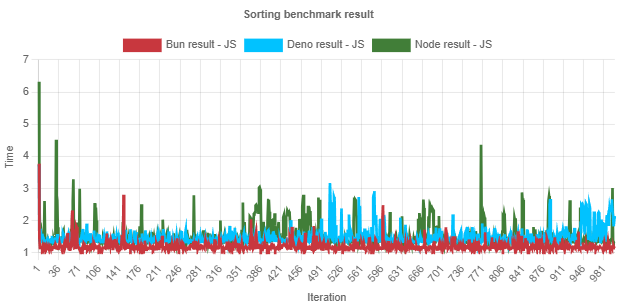
\includegraphics[width=0.8\textwidth]{Figures/sorting/bubble/e3_js.png}
  \caption{Wyniki eksperymentów dla algorytmu sortowania bąbelkowego dla 1000 iteracji i 1000 elementów}
  \label{fig:bubble_sorting_e3}
\end{figure}

Na wykresie \ref{fig:bubble_sorting_e3_memory_js} przedstawiono wyniki eksperymentów dla algorytmu sortowania bąbelkowego dla 1000 iteracji oraz 1000 elementów napisanego w języku JavaScript. Na osi X przedstawiono liczbę iteracji, natomiast na osi Y wykorzystanie pamięci w kilobytach. Jak widać, czas wykonania algorytmu rośnie wraz z ilością elementów.
\begin{figure}[H]
  \centering
  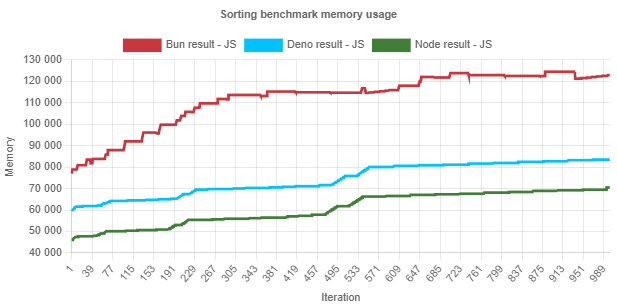
\includegraphics[width=0.8\textwidth]{Figures/sorting/bubble/e3_memory_js.png}
  \caption{Wyniki eksperymentów dla algorytmu sortowania bąbelkowego dla 1000 iteracji i 1000 elementów}
  \label{fig:bubble_sorting_e3_memory_js}
\end{figure}

Na wykresie \ref{fig:bubble_sorting_e3_ts} przedstawiono wyniki eksperymentu dla 1000 iteracji oraz 1000 elementów dla algorytmów sortowania bąbelkowego, napisanego w języku TypeScript. Na osi X przedstawia liczbę iteracji, na osi Y czas wykonania algorytmu w sekundach. 

\begin{figure}[H]
  \centering
  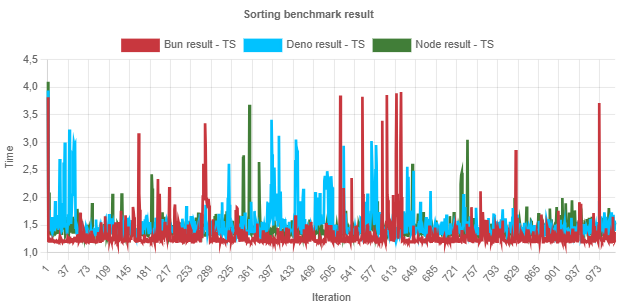
\includegraphics[width=0.8\textwidth]{Figures/sorting/bubble/e3_ts.png}
  \caption{Wyniki eksperymentów dla algorytmu sortowania bąbelkowego dla 1000 iteracji i 1000 elementów}
  \label{fig:bubble_sorting_e3_ts}
\end{figure}

Na wykresie \ref{fig:bubble_sorting_e3_memory_ts} przedstawiono wyniki eksperymentów dla algorytmu sortowania bąbelkowego. Na osi X przedstawiono liczbę iteracji, natomiast na osi Y wykorzystanie pamięci w kilobytach. Jak widać, czas wykonania algorytmu rośnie wraz z ilością elementów.
\begin{figure}[H]
  \centering
  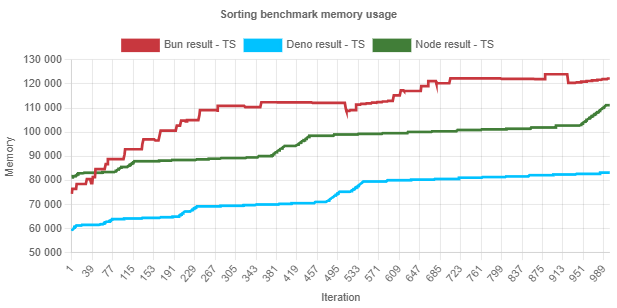
\includegraphics[width=0.8\textwidth]{Figures/sorting/bubble/e3_memory_ts.png}
  \caption{Wyniki eksperymentów dla algorytmu sortowania bąbelkowego dla 1000 iteracji i 1000 elementów}
  \label{fig:bubble_sorting_e3_memory_ts}
\end{figure}

%4
Na wykresie \ref{fig:bubble_sorting_e4} przedstawiono wyniki eksperymentów dla algorytmu sortowania bąbelkowego. Na osi X przedstawiono liczbę iteracji, natomiast na osi Y wykorzystanie pamięci w kilobytach. Jak widać, czas wykonania algorytmu rośnie wraz z ilością elementów.
\begin{figure}[H]
  \centering
  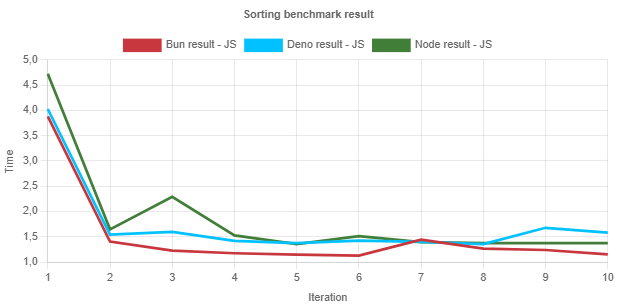
\includegraphics[width=0.8\textwidth]{Figures/sorting/bubble/e4_js.png}
  \caption{Wyniki eksperymentów dla algorytmu sortowania bąbelkowego dla 10 iteracji i 10000 elementów}
  \label{fig:bubble_sorting_e4}
\end{figure}

Na wykresie \ref{fig:bubble_sorting_e4_memory_js} przedstawiono wyniki eksperymentów dla algorytmu sortowania bąbelkowego. Na osi X przedstawiono liczbę iteracji, natomiast na osi Y wykorzystanie pamięci w kilobytach. Jak widać, czas wykonania algorytmu rośnie wraz z ilością elementów.
\begin{figure}[H]
  \centering
  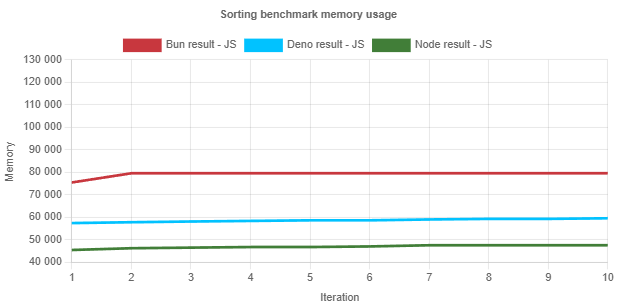
\includegraphics[width=0.8\textwidth]{Figures/sorting/bubble/e4_memory_js.png}
  \caption{Wyniki eksperymentów dla algorytmu sortowania bąbelkowego dla 10 iteracji i 10000 elementów}
  \label{fig:bubble_sorting_e4_memory_js}
\end{figure}

Na wykresie \ref{fig:bubble_sorting_e4_ts} przedstawiono wyniki eksperymentu dla 100 iteracji oraz 1000 elementów dla algorytmów sortowania bąbelkowego. Na osi X przedstawia liczbę iteracji, na osi Y czas wykonania algorytmu w sekundach. 

\begin{figure}[H]
  \centering
  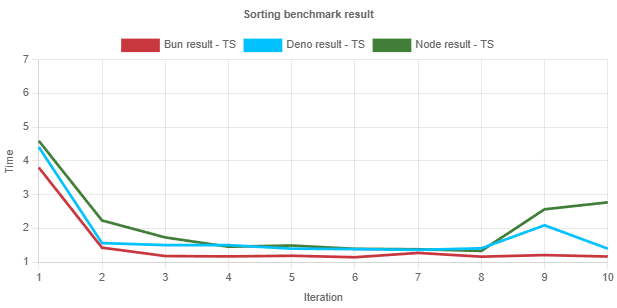
\includegraphics[width=0.8\textwidth]{Figures/sorting/bubble/e4_ts.png}
  \caption{Wyniki eksperymentów dla algorytmu sortowania bąbelkowego dla 10 iteracji i 10000 elementów}
  \label{fig:bubble_sorting_e4_ts}
\end{figure}

Na wykresie \ref{fig:bubble_sorting_e4_memory_ts} przedstawiono wyniki eksperymentów dla algorytmu sortowania bąbelkowego. Na osi X przedstawiono liczbę iteracji, natomiast na osi Y wykorzystanie pamięci w kilobytach. Jak widać, czas wykonania algorytmu rośnie wraz z ilością elementów.
\begin{figure}[H]
  \centering
  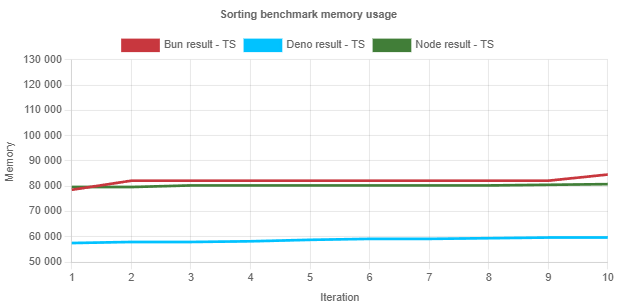
\includegraphics[width=0.8\textwidth]{Figures/sorting/bubble/e4_memory_ts.png}
  \caption{Wyniki eksperymentów dla algorytmu sortowania bąbelkowego dla 10 iteracji i 10000 elementów}
  \label{fig:bubble_sorting_e4_memory_ts}
\end{figure}

% 5
Na wykresie \ref{fig:bubble_sorting_e5} przedstawiono wyniki eksperymentów dla algorytmu sortowania bąbelkowego. Na osi X przedstawiono liczbę iteracji, natomiast na osi Y wykorzystanie pamięci w kilobytach. Jak widać, czas wykonania algorytmu rośnie wraz z ilością elementów.
\begin{figure}[H]
  \centering
  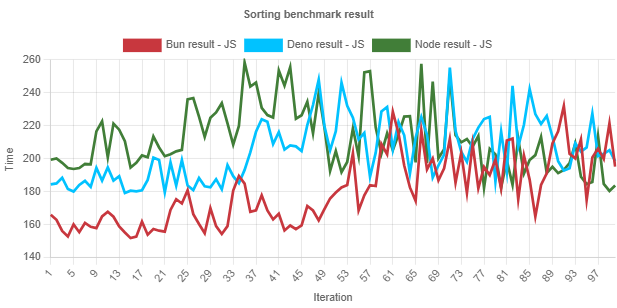
\includegraphics[width=0.8\textwidth]{Figures/sorting/bubble/e5_js.png}
  \caption{Wyniki eksperymentów dla algorytmu sortowania bąbelkowego dla 100 iteracji i 10000 elementów}
  \label{fig:bubble_sorting_e5}
\end{figure}

Na wykresie \ref{fig:bubble_sorting_e5_memory_js} przedstawiono wyniki eksperymentów dla algorytmu sortowania bąbelkowego. Na osi X przedstawiono liczbę iteracji, natomiast na osi Y wykorzystanie pamięci w kilobytach. Jak widać, czas wykonania algorytmu rośnie wraz z ilością elementów.
\begin{figure}[H]
  \centering
  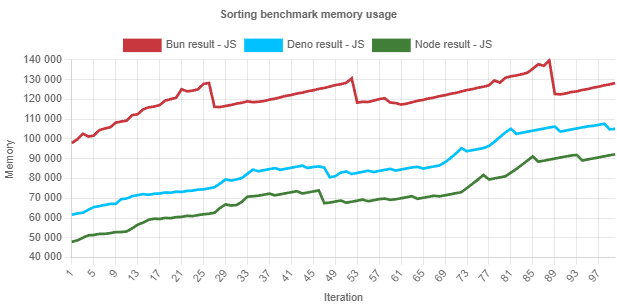
\includegraphics[width=0.8\textwidth]{Figures/sorting/bubble/e5_memory_js.png}
  \caption{Wyniki eksperymentów dla algorytmu sortowania bąbelkowego dla 100 iteracji i 10000 elementów}
  \label{fig:bubble_sorting_e5_memory_js}
\end{figure}

Na wykresie \ref{fig:bubble_sorting_e5_ts} przedstawiono wyniki eksperymentu dla 100 iteracji oraz 1000 elementów dla algorytmów sortowania bąbelkowego. Na osi X przedstawia liczbę iteracji, na osi Y czas wykonania algorytmu w sekundach. 

\begin{figure}[H]
  \centering
  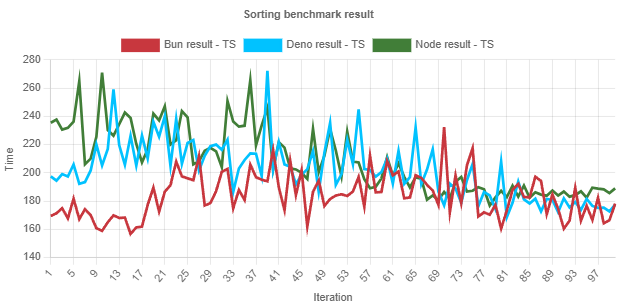
\includegraphics[width=0.8\textwidth]{Figures/sorting/bubble/e5_ts.png}
  \caption{Wyniki eksperymentów dla algorytmu sortowania bąbelkowego dla 100 iteracji i 10000 elementów}
  \label{fig:bubble_sorting_e5_ts}
\end{figure}

Na wykresie \ref{fig:bubble_sorting_e5_memory_ts} przedstawiono wyniki eksperymentów dla algorytmu sortowania bąbelkowego. Na osi X przedstawiono liczbę iteracji, natomiast na osi Y wykorzystanie pamięci w kilobytach. Jak widać, czas wykonania algorytmu rośnie wraz z ilością elementów.
\begin{figure}[H]
  \centering
  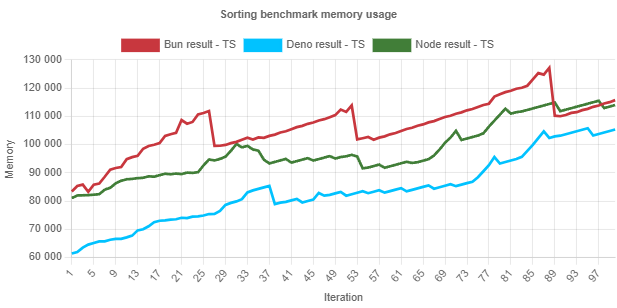
\includegraphics[width=0.8\textwidth]{Figures/sorting/bubble/e5_memory_ts.png}
  \caption{Wyniki eksperymentów dla algorytmu sortowania bąbelkowego dla 100 iteracji i 10000 elementów}
  \label{fig:bubble_sorting_e5_memory_ts}
\end{figure}

% 6
Na wykresie \ref{fig:bubble_sorting_e6} przedstawiono wyniki eksperymentów dla algorytmu sortowania bąbelkowego. Na osi X przedstawiono liczbę iteracji, natomiast na osi Y wykorzystanie pamięci w kilobytach. Jak widać, czas wykonania algorytmu rośnie wraz z ilością elementów.
\begin{figure}[H]
  \centering
  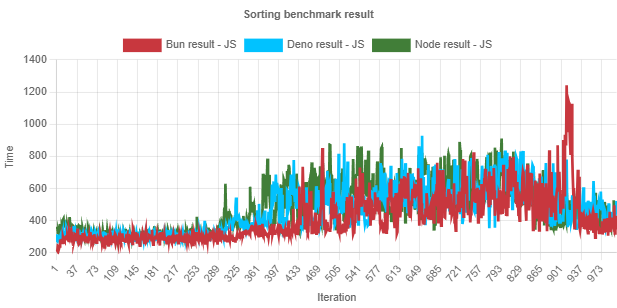
\includegraphics[width=0.8\textwidth]{Figures/sorting/bubble/e6_js.png}
  \caption{Wyniki eksperymentów dla algorytmu sortowania bąbelkowego dla 1000 iteracji i 10000 elementów}
  \label{fig:bubble_sorting_e6}
\end{figure}

Na wykresie \ref{fig:bubble_sorting_e6_memory_js} przedstawiono wyniki eksperymentów dla algorytmu sortowania bąbelkowego. Na osi X przedstawiono liczbę iteracji, natomiast na osi Y wykorzystanie pamięci w kilobytach. Jak widać, czas wykonania algorytmu rośnie wraz z ilością elementów.
\begin{figure}[H]
  \centering
  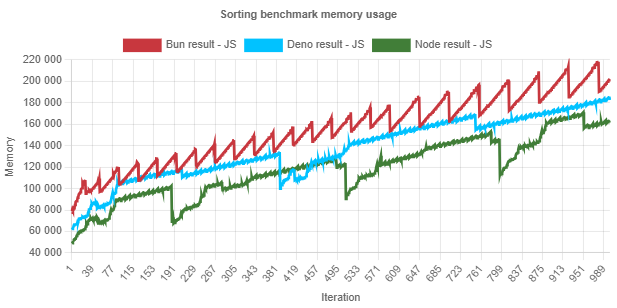
\includegraphics[width=0.8\textwidth]{Figures/sorting/bubble/e6_memory_js.png}
  \caption{Wyniki eksperymentów dla algorytmu sortowania bąbelkowego dla 1000 iteracji i 10000 elementów}
  \label{fig:bubble_sorting_e6_memory_js}
\end{figure}

Na wykresie \ref{fig:bubble_sorting_e6_ts} przedstawiono wyniki eksperymentu dla 100 iteracji oraz 1000 elementów dla algorytmów sortowania bąbelkowego. Na osi X przedstawia liczbę iteracji, na osi Y czas wykonania algorytmu w sekundach. 

\begin{figure}[H]
  \centering
  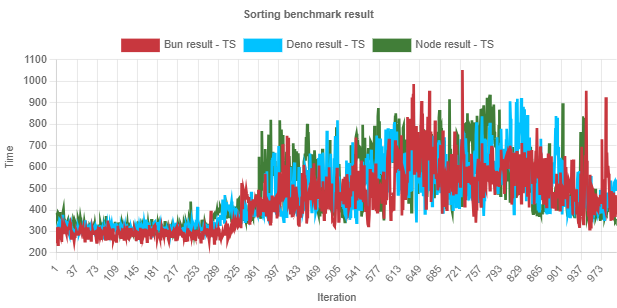
\includegraphics[width=0.8\textwidth]{Figures/sorting/bubble/e6_ts.png}
  \caption{Wyniki eksperymentów dla algorytmu sortowania bąbelkowego dla 1000 iteracji i 10000 elementów}
  \label{fig:bubble_sorting_e6_ts}
\end{figure}

Na wykresie \ref{fig:bubble_sorting_e6_memory_ts} przedstawiono wyniki eksperymentów dla algorytmu sortowania bąbelkowego. Na osi X przedstawiono liczbę iteracji, natomiast na osi Y wykorzystanie pamięci w kilobytach. Jak widać, czas wykonania algorytmu rośnie wraz z ilością elementów.
\begin{figure}[H]
  \centering
  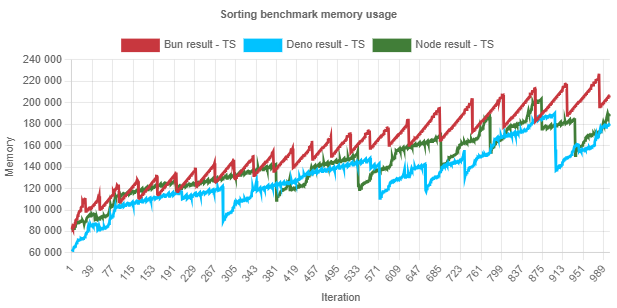
\includegraphics[width=0.8\textwidth]{Figures/sorting/bubble/e6_memory_ts.png}
  \caption{Wyniki eksperymentów dla algorytmu sortowania bąbelkowego dla 1000 iteracji i 10000 elementów}
  \label{fig:bubble_sorting_e6_memory_ts}
\end{figure}

\subsubsection{Wyniki - sortowanie szybkie}

\subsubsection{Wyniki - sortowanie pozycyjne}

\subsection{Algorytmy kodowania}

\subsubsection{Wyniki}

\subsection{Testy wydajnościowe operacji zapisu i odczytu plików}

\subsubsection{Wyniki}

\subsection{Testy wydajnościowe serwera HTTP}

\subsubsection{Wyniki}

\subsection{Testy wydajnościowe zapisu i odczytu danych z bazy danych}

\subsubsection{Wyniki}

\newpage
\section{Dyskusja wyników}
W tym rozdziale została przedstawiona dyskusja wniosków na temat wyników przeprowadzonych podczas badań. Pokazują one jak zachowują się środowiska w różnych sytuacjach, jakie są różnice między nimi oraz pokazują ich wady i zalety. Dodatkowo zostały porównane istniejącymi wynikami, które znajdują się w przeglądzie środowisk oraz literatury.

\subsection{Algorytmy sortowania}
Testowanie algorytmów sortowania pokazało iż testy zostały przeprowadzone poprawnie, zaobserwowano zachowania środowisk, które prowadzą do wniosku, że algorytmy sortowania zachowują się zgodnie z przewidywaniami. Algorytmy sortowania szybkiego i bąbelkowego są algorytmami o złożoności obliczeniowej $O(n^2)$, co potwierdzają wyniki testów. Algorytm sortowania pozycyjnego jest algorytmem o złożoności obliczeniowej $O(nk)$, gdzie $k$ jest ilością możliwych wartości w tablicy, co potwierdzają wyniki testów.

Algorytm sortowania szybkiego jest zdecydowanie szybszy od algorytmu bąbelkowego, co jest zgodne z przewidywaniami. Algorytm sortowania szybkiego jest zdecydowanie szybszy od algorytmu bąbelkowego, co jest zgodne z przewidywaniami. Sortowanie szybkie zaobserwowano pesymistyczny wykonanie algorytmu, w której pamięć w sposób rekurencyjny, powoduje to dość szybkie zapełnienie pamięci. Zjawisko zostało zaobserwowano w szczególności przy środowisku Bun, w którym zużycie pamięci wzrasta liniowo. Środowisko zostało napisane w języku Zig, które nie posiada zaimplementowanych przez język możliwości zwalniania pamięci, co powoduje, że pamięć nie jest zwalniana w sposób optymalny. 

W przypadku pozostałych środowisk zaobserwowano mniejsze zużycie pamięci operacyjnej, pozwala to na wysnucie wniosku o lepiej zoptymalizowanym przez twórców środowiska. Zaobserwowano również zjawisko rozgrzewania się silnika JavaScript, polega ono na rozpoczęciu buforowanie zawartości stosu wywołań, co pozwala na szybsze wykonanie kodu. Zjawisko to jest zauważalne w przypadku środowiska Node.js, w którym pierwsze wykonanie algorytmu sortowania szybkiego jest wolniejsze od kolejnych.

Przy wykonywaniu testów na algorytmie sortowania szybkiego zaobserwowano zjawisko, w który środowisko Bun jest zdecydowanie wolniejsze od pozostałych oraz daje nieregularne wyniki. Tym zjawiskiem jest rekurencja, możemy zauważyć, że Bun posiada rygorystyczny algorytm Garbage Collector, który zwalnia dużo pamięci usuwając obiekty, które nie są już używane. W wynikach widzimy spadki używanej pamięci przez proces, co przekłada się na ponowne alokowanie pamięci, co spowodowało wydłużenie wykonania algorytmu sortowania. W porównaniu do innych środowisk, które nie posiadają tak rygorystycznego algorytmu Garbage Collector, co pozwala na szybsze wykonanie algorytmu sortowania oraz mniejsze zużycie pamięci. 

Na samym repozytorium środowiska Bun możemy zauważyć dużo zgłoszonych przez użytkowników środowiska błędów dotyczący zużycia pamięci, co potwierdza nasze obserwacje \cite{bun_memory}. Pozostałe środowiska poprzez bazowanie na silniku V8, posiadają mniejszą liczbę związanych z pamięcią błędów, co pozwala na szybsze wykonanie algorytmu sortowania oraz mniejsze zużycie pamięci.

\subsection{Algorytm kodowania \textit{Base64}}
Testy przeprowadzone na kodowaniu za pomocą algorytmu Base64 zostały przeprowadzone poprawnie, zaobserwowano zachowania środowisk, które prowadzą do wniosku, że algorytmy kodowania zachowują się zgodnie z przewidywaniami. Algorytm kodowania \textit{Base64} jest algorytmem o złożoności obliczeniowej $O(n)$, co potwierdzają wyniki testów. W porównaniu do operacji dekodowania wykonuje się dłużej, ze względu na zwiększenie rozmiaru danych, co przekłada się na dłuższy czas wykonywania operacji. Operacja dekodowania jest zdecydowanie wolniejsza od operacji kodowania, co jest zgodne z przewidywaniami, ze względu na zwiększenie rozmiaru.

Testy pokazały zbliżone wyniki, kodowanie w środowiskach NodeJS oraz Bun były zdecydowanie szybsze niż Deno. Wynika to z faktu implementacji operacji kodowania w środowisku Deno, w przeciwieństwie do środowisk NodeJS oraz Bun, które posiadają szybszą implementację operacji kodowania z wykorzystaniem biblioteki standardowej \textit{Buffer}. Bezpośrednio wpływa na czas wykonania, a dodatkowo nie wpływa na zużycie pamięci operacyjnej. Dodatkowo możemy zauważyć, że środowisko Deno zmniejsza czasu wykonania operacji dekodowania w porównaniu do środowiska NodeJS oraz Bun, gdzie wyniki pozostałych środowisk są zbliżone.

Zużycie pamięci w testu dekodowania jest zdecydowanie większe niż w przypadku kodowania, co jest zgodne z przewidywaniami. W przypadku środowiska NodeJS możemy odnotować najmniejsze zużycie pamięci operacyjnej, co wynika z optymalizacji biblioteki standardowej \textit{Buffer}. W przypadku środowiska Bun jest zdecydowanie większe zużycie pamięci operacyjnej, co wynika z licznych błędów związanych z wyciekami pamięci, które zostały zgłoszone przez użytkowników \cite{bun_memory}. W przypadku środowiska Deno zużycie pamięci operacyjnej jest zdecydowanie większe niż w przypadku środowiska NodeJS, co wynika z implementacji operacji dekodowania w środowisku Deno.

\subsection{Testy wydajnościowe operacji zapisu i odczytu pliku}
Testy wydajnościowe operacji zapisu i odczytu pliku pokazały, że operacje zapisu i odczytu pliku są zależne od środowiska, w którym są wykonywane. W przypadku operacji zapisu pliku, środowisko Deno jest zdecydowanie szybsze od środowiska NodeJS oraz Bun. Wynika to z faktu, że środowisko Deno posiada własną implementacje obiektu pliku, która wykazała w testach, że jest szybsza niż pozostałe środowiska.

W przypadku operacji odczytu pliku środowiska Deno oraz NodeJS są zdecydowanie szybsze od środowiska Bun, wynika to z faktu posiadania wspólnego silnika JavaScript, w którym operacje odczytu pliku są zoptymalizowane. W przypadku środowiska Bun, który bazuje na silniku WebKit, operacje odczytu pliku są wolniejsze, co potwierdziły testy. Zaobserwowano również liniowe zwiększanie pamięci, podczas odczytywania plików ze względu na alokowanie pamięci na dane z danego pliku. Zachowanie to jest zgodne z przewidywaniami, w przypadku operacji odczytu pliku.

W przeciwieństwie do operacji odczytu pliku, operacja zapisu jest zdecydowanie bardziej obciążająca środowiska. Przy każdym z testów zostaje generowane nowe pliki tekstowe, które różnią się zawartością, co wywołuje także trzymanie ich zawartości w pamięci podręcznej. Z tego względu wykonanie takiego testu jest bardziej obciążające dla środowiska, co potwierdzają wyniki testów. Największe zużycie pamięci możemy zobaczyć w przypadku środowiska Bun, które posiada dużo zgłoszonych błędów związanych z pamięcią \cite{bun_memory}. Dodatkowo w przypadku tego środowiska została wykorzystana jego własnej implementacji obiektu pliku. W przypadku środowiska NodeJS oraz Deno zużycie pamięci jest mniejsze, co wynika z optymalizacji operacji zapisu pliku.

Porównując wyniki testów operacji zapisu i odczytu pliku, możemy zauważyć, że operacja zapisu pliku jest bardziej obciążająca dla środowiska niż operacja odczytu pliku. Wynika to z faktu, że operacja zapisu pliku wymaga alokacji pamięci na dane, które mają zostać zapisane, co powoduje zwiększenie zużycia pamięci operacyjnej. W przypadku operacji odczytu pliku, dane są odczytywane z pliku, co nie wymaga alokacji pamięci na dane, co przekłada się na mniejsze zużycie pamięci operacyjnej.

\subsection{Testy obciążeniowe serwera HTTP}
Testy wydajnościowe serwerów HTTP pokazały, że pozyskiwane wartości RPS (ang. \textit{Request per second}) różnią się w zależności od środowiska, w którym zostały stworzone. Program Oha \cite{oha} pozwolił na dokładne zmierzenie tych wartości RPS oraz ich porównanie, wszystkie parametry zostały ustawione tak samo dla każdego środowiska. Wadą programu Oha jest to, że nie pozwala na zmierzenie zużycia pamięci oraz obciążenia procesora, co jest wyznacznikiem obciążenia danego serwera.

Wyniki testów pokazały, że środowisko Deno jest zdecydowanie szybsze od środowiska NodeJs oraz Bun. Posiada on najwyższy wynik wyrażony w RPS, co wynika z faktu, że środowisko Deno bazuje na silniku V8, który jest zoptymalizowany pod kątem wydajności. W przypadku środowiska NodeJS ma ono podobne wyniki do środowiska Deno, co wynika z faktu, że oba środowiska bazują na silniku V8. W przypadku środowiska Bun, które bazuje na silniku WebKit, wyniki są zdecydowanie gorsze od pozostałych środowisk. Wynika to z faktu, że silnik WebKit nie jest zoptymalizowany pod kątem wydajności, co potwierdzają wyniki testów.

Testy wykazały także, że wyniki, które przedstawił twórca Bun w \cite{bun_test} nie potwierdziły się zgodnie z jego przewidywaniami. Twórca środowiska Bun przewidywał, że środowisko Bun będzie zdecydowanie szybsze od środowiska NodeJS oraz Deno. Wyniki testów pokazały, że środowisko Bun jest zdecydowanie wolniejsze od środowiska NodeJS oraz Deno. Pokazuje to fakt, że młode środowisko jakim jest Bun, nie jest jeszcze zoptymalizowane pod kątem wydajności, co potwierdzają wyniki testów.

\subsection{Testy wydajnościowe zapisu i odczytu z bazy danych}
Testy wydajnościowe zapisu i odczytu z bazy danych pokazały, że operacje zapisu i odczytu z bazy danych są zależne od środowiska, w którym są wykonywane. W przypadku operacji zapisu do bazy danych, środowisko Deno jest zdecydowanie szybsze od środowiska NodeJS oraz Bun. Wynika to z faktu, że środowisko Deno posiada własną implementacje obiektu bazy danych, która wykazała w testach, że jest szybsza niż pozostałe środowiska. Dodatkowo środowisko Deno posiada wbudowaną obsługę bazy danych SQLite, co pozwala na szybsze wykonanie operacji zapisu do bazy danych.

W przypadku operacji odczytu z bazy danych środowiska Deno oraz NodeJS są zdecydowanie szybsze od środowiska Bun, wynika to z faktu posiadania wspólnego silnika JavaScript, w którym operacje odczytu z bazy danych są zoptymalizowane. W przypadku środowiska Bun, który bazuje na silniku WebKit, operacje odczytu z bazy danych są wolniejsze, co potwierdziły testy. Zaobserwowano również, że Bun posiada zdecydowanie większe zużycie pamięci operacyjnej, co wynika z licznych błędów związanych z pamięcią \cite{bun_memory}. W przypadku środowiska NodeJS oraz Deno zużycie pamięci jest mniejsze, co wynika z optymalizacji operacji odczytu z bazy danych.

Natomiast w przypadku zapisu do bazy danych, zużycie pamięci jest zdecydowanie większe niż w przypadku odczytu z bazy danych, co jest zgodne z przewidywaniami. W przypadku operacji zapisu do bazy danych, dane są zapisywane do bazy danych, co wymaga alokacji pamięci na dane, co przekłada się na zwiększenie zużycia pamięci operacyjnej. W przypadku operacji odczytu z bazy danych, dane są odczytywane z bazy danych, co nie wymaga alokacji pamięci na dane, co przekłada się na mniejsze zużycie pamięci operacyjnej.

W przypadku zwiększenia ilości rekordów zaobserwowano zwiększenie czasu wykonania operacji zapisu oraz odczytu z bazy danych. Wynika to z faktu, że zwiększenie powoduje zwiększenie ilości danych, które muszą być zapisane lub odczytane z bazy danych, co przekłada się na zwiększenie czasu wykonania operacji. W przypadku zwiększenia ilości rekordów, zużycie pamięci operacyjnej również wzrasta, co jest zgodne z przewidywaniami. Testy zostały przeprowadzone na plikowej bazie danych, co mogło wpłynąć na wyniki testów, w przypadku baz relacyjnych, które mogą być umieszczone na zewnętrznym serwerze, aby odciążyć maszynę, na której wykonywane są testy.


\newpage
\section{Podsumowanie}


% Wykaz literatury
\newpage
\bibliographystyle{apalike}
\bibliography{literatura.bib}

% Inne spisy
\newpage
\listoffigures
\newpage
\listoftables
\newpage
\listofmyequations
\newpage
\renewcommand{\lstlistlistingname}{Spis kodów}
\lstlistoflistings

\newpage
\section*{Wykaz symboli i oznaczeń}
\subsection*{Symbole łacińskie}

\subsection*{Symbole greckie}

\subsection*{Indeksy i wskaźniki}

\subsection*{Skróty}

\nomenclature{WWW}{World Wide Web}
\nomenclature{RAM}{Random Access Memory}
\nomenclature{HTTP}{Hypertext Transfer Protocol}

\printnomenclature

\newpage
\section*{Wykaz używanych skrótów}
\begin{itemize}
  \item \textbf{WWW} (ang. \textit{World Wide Web})
  \item \textbf{RAM} (ang. \textit{Random Access Memory})
  \item \textbf{HTTP} (ang. \textit{Hypertext Transfer Protocol})
\end{itemize}

\newpage
\section*{Wykaz definicji}

\newpage
\section*{Wykaz załączników}


\end{document}
